\documentclass{article}

\usepackage[english]{babel}

\usepackage[letterpaper,top=2cm,bottom=2cm,left=3cm,right=3cm,marginparwidth=1.75cm]{geometry}

% Useful packages
\usepackage{amsmath}
\usepackage{graphicx}
\usepackage{subfig}
\usepackage[colorlinks=true, allcolors=blue]{hyperref}

\title{Music Genre Analysis}
\author{Rohan Kumar Sah}

\begin{document}
\maketitle

\begin{abstract}
This report was written to explain my thought process and methodology and to compile all the aiding visualisations and results in one place for KDAG 2025 Selections - Core Team Task 2. Please refer to the notebook as all the code is explained there first. I will avoid including any code in this report.
\end{abstract}

\section{Introduction}

Each sub-task is discussed in a separate section.
The libraries used are as follows : 
\begin{itemize}
\item pandas : for interacting with the dataset
\item numpy : for making life easier
\item seaborn + matplotlib : for visualisation
\item random : for initialising centroids in clustering algorithm
\end{itemize}

\section{Vectorisation}

For generating embeddings, we were supposed to choose between BoW (Bag of Words) and TF-IDF. I went with BoW for the following reasons :
\begin{itemize}
\item BoW is extremely simple to implement and performs well for small datasets like this one.
\item TF-IDF would have been a better choice if we were working with a text corpus but for this keyword analysis BoW does the trick.
\item TF-IDF would recognise common words and reduce their impact, but here each keyword is equally important.

\begin{table}
\centering
\begin{tabular}{l|r}
keyword\_1 & Frequency \\\hline
banjo & 6 \\
brass & 11 \\
guitar & 65 \\
piano & 12 \\
synth & 43 \\
violin & 10
\end{tabular}
\caption{\label{tab:widgets} keyword\_1 and frequency comparison}
\end{table}

It would be silly to discriminate between guitar and violin - see Table 1, because of frequency since there is no semantics involved here due to the dataset being three keywords, and TF-IDF doesn't serve its purpose well.
\end{itemize}


\section{Dimensionality reduction}
This involves standard PCA code using numpy. We simplified the sparse vectors while retaining helpful information.

\section{Combining the embeddings into one}
There are multiple ways of combining embeddings.
Concatenation is out of the question since we are trying to preserve the dimensions. Since all keywords are equally important, we averaged the vectors. Simply summing up can cause larger magnitudes we do not want to deal with.
\[
V_{\text{final}} = \frac{1}{3} \sum_{i=1}^{3} V_i
\]
Cross Product would collapse the vector into a scalar, and we would lose information. For K-Means (which we will implement in the next section), average is the best choice.
\begin{figure}[h]
    \centering
    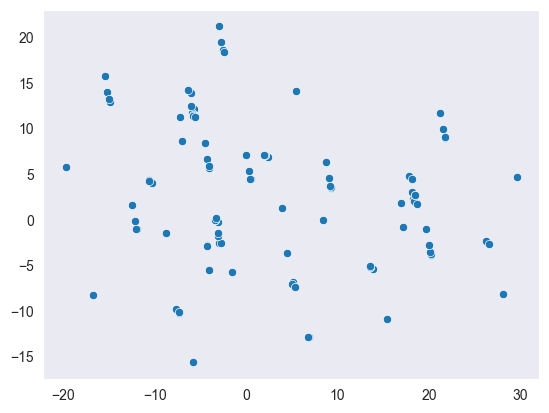
\includegraphics[width=1\textwidth]{vecs.png} % Adjust width as needed
    \caption{Vectors after combination}
    \label{fig:vectors}
\end{figure}
\pagebreak
\section{Clustering}
I started with the K-Means algorithm for clustering; looking at the WCSS (Within-Cluster Sum of Square) and Silhouette Scores for different cluster numbers gives an idea of what value to take. Looking at the Elbow Point in the graph and considering that there are five genres means we should take k=5 for further analysis.
\begin{figure}[h]
    \centering
    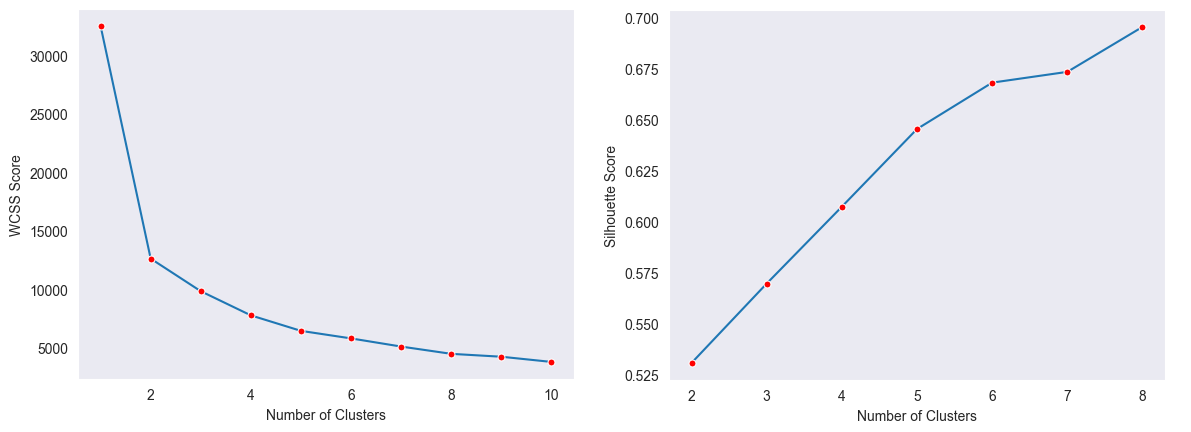
\includegraphics[width=1\textwidth]{metrics.png}
    \caption{Metrics averaged over 100 iterations}
    \label{fig:metrics}
\end{figure}

However, soon, a problem arises: the K-Means algorithm can sometimes be inaccurate. Since the centroids are randomly initialised, if a centroid is initialised too far from the points, it won't shift, and if two centroids are initialised too close, they probably won't move.

\begin{figure}[h]
    \centering
    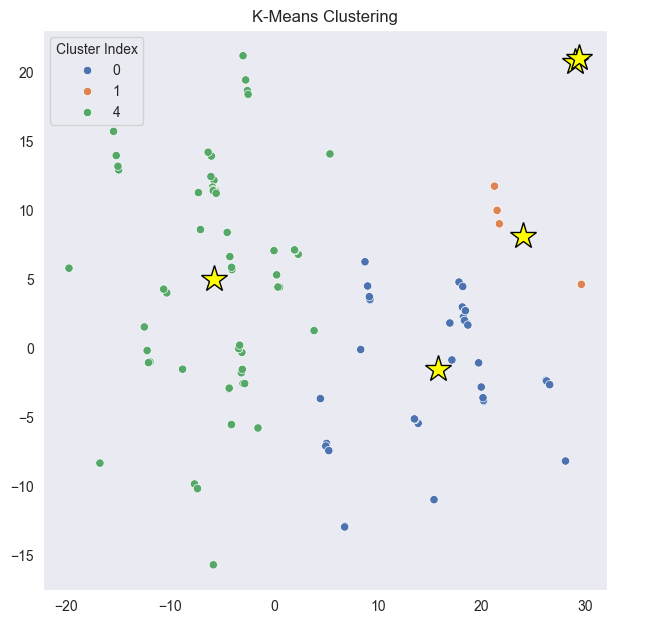
\includegraphics[width=0.5\textwidth]{fail.png} % Adjust width as needed
    \caption{A failed K-Means example where two centroids are at a corner and belong to no cluster}
    \label{fig:failure}
\end{figure}
The problem lies in centroid initialisation, so we must find a better way. We, therefore, shift to K-Means++, where centroids are initialised iteratively. Failures are almost eliminated by this method.
\begin{figure}[h]
    \centering
    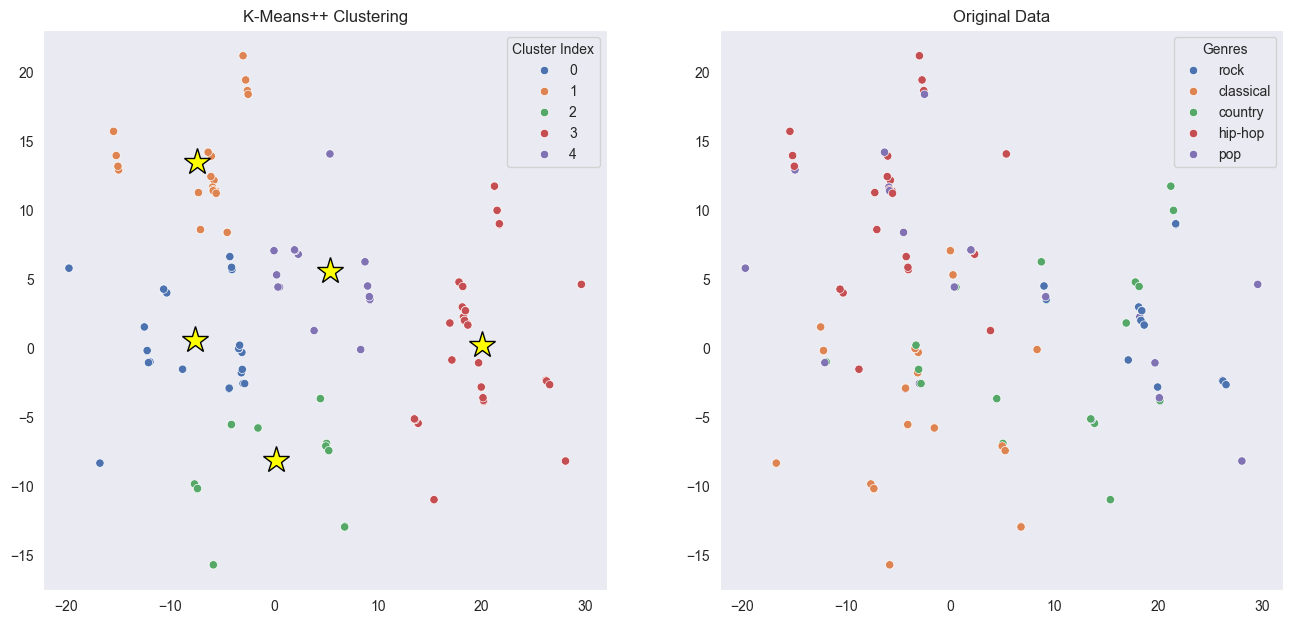
\includegraphics[width=0.9\textwidth]{output.png} % Adjust width as needed
    \caption{Final Clustering}
    \label{fig:output}
\end{figure}
\pagebreak
\section{Analysis}
\subsection{Percentage distribution of ground truth genres in each cluster}
We plot a heatmap, comparing percentages of the genres within each cluster.
\begin{figure}[h]
    \centering
    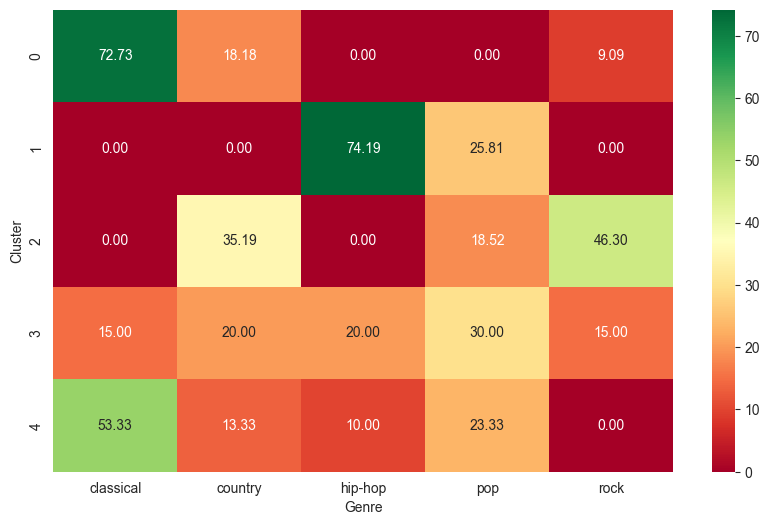
\includegraphics[width=0.7\textwidth]{heatmap.png} % Adjust width as needed
    \caption{Heatmap showing the percentages of different genres within each cluster}
    \label{fig:distribution}
\end{figure}
We observe the following :
\begin{itemize}
\item Cluster 0 is mostly populated by Classical (72.73\%)
\item Cluster 1 is mostly populated by Hip-Hop (74.19\%)
\item Cluster 2 is not dominated by a single genre
\item Cluster 3 has a more even distribution then Cluster 2
\item Cluster 4 is also mostly classical
\end{itemize}
\pagebreak
\begin{figure}[h]
    \centering
    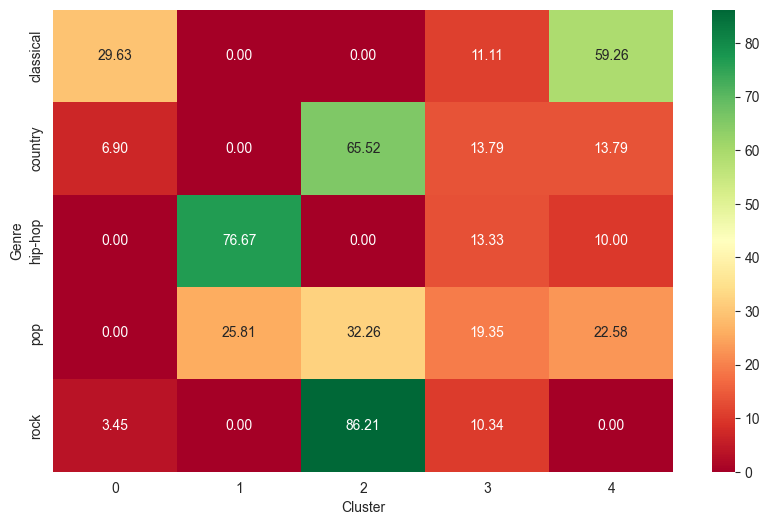
\includegraphics[width=0.7\textwidth]{heatmap2.png} % Adjust width as needed
    \caption{Heatmap showing the percentage of songs from each genre in each cluster}
    \label{fig:distributionreverse}
\end{figure}
If we switch our calculation a bit we observe something else as well. Rock is the best clustered genre because most of its points are within the same genre. The Clustering of Hip-Hop and Country is also not that bad. Pop is the most poorly clustered of all.
\subsection{Silhouette Score}
We already have the general idea of the Silhouette Score for different number of clusters - see Figure 2.
The silhouette score for a single sample is defined as:

\[
s(i) = \frac{b(i) - a(i)}{\max(a(i), b(i))}
\]

where:
\begin{itemize}
    \item \( a(i) \) is the average intra-cluster distance (mean distance to other points in the same cluster).
    \item \( b(i) \) is the average nearest-cluster distance (mean distance to points in the nearest neighboring cluster).
\end{itemize}

The average silhouette score for 5 clusters over 100 iterations is:

\[
\text{Average Silhouette Score} = 0.65460999
\]

For most iterations with k=5, the silhouette score remains within the range:

\[
0.6 \leq s \leq 0.7
\]

where \( s \) represents the silhouette score.
This is a good clustering score considering that we used the most simplistic approaches to the problems in this task.

\subsection{Genre Prediction}
On converting the keywords to vectors and finding the nearest centroid we obtain the following results
\begin{itemize}
    \item \texttt{['piano', 'calm', 'slow']} belongs to cluster 2
    \item \texttt{['guitar', 'emotional', 'distorted']} belongs to cluster 0
    \item \texttt{['synth', 'mellow', 'distorted']} belongs to cluster 1
\end{itemize}
\pagebreak
We can refer to Figure 5 and make the following observations : 
\begin{itemize}
\item Cluster 2 is not really dominated by a single genre but we can sort \texttt{['piano', 'calm', 'slow']} into Country
\item Cluster 0 is dominated by Classical so we can sort \texttt{['guitar', 'emotional', 'distorted']} into Classical
\item Cluster 1 is dominated by hip-Hop so we can sort \texttt{['synth', 'mellow', 'distorted']} into Hip-Hop
\end{itemize}


\end{document}